\label{sec:analysis}
We now study \method{} from a graph convolution perspective. We demonstrate that \method{} corresponds to a fixed filter on the graph spectral domain. 
In addition, we show that adding self-loops to the original graph, i.e. the renormalization trick \citep{gcn}, effectively shrinks the underlying graph spectrum.
On this scaled domain, \method{} acts as a low-pass filter that produces smooth features over the graph. As a result, nearby nodes tend to share similar representations and consequently predictions.


\subsection{Preliminaries on Graph Convolutions}
Analogous to the Euclidean domain, graph Fourier analysis relies on the spectral decomposition of graph Laplacians. The graph Laplacian $\boldsymbol{\Delta} = \rmD - \rmA$ (as well as its normalized version $\boldsymbol{\Delta}_{\text{sym}} = \rmD^{-1/2}\boldsymbol{\Delta} \rmD^{-1/2}$) is a symmetric positive semidefinite matrix with eigendecomposition $\boldsymbol{\Delta} = \rmU \boldsymbol{\Lambda} \rmU^{\top}$, where $\rmU \in \mathbb{R}^{n \times n}$ comprises orthonormal eigenvectors and $\boldsymbol{\Lambda} = \text{diag}(\lambda_1, \dots, \lambda_n)$ is a diagonal matrix of eigenvalues. The eigendecomposition of the Laplacian allows us to define the Fourier transform equivalent on the graph domain, where eigenvectors denote Fourier modes and eigenvalues denote frequencies of the graph. In this regard, let $\rvx \in \mathbb{R}^n$ be a signal defined on the vertices of the graph. We define the graph Fourier transform of $\rvx$ as $\hat{\rvx} = \rmU^{\top}\rvx$, with inverse operation given by $\rvx = \rmU \hat{\rvx}$.
Thus, the graph convolution operation between signal $\rvx$ and filter $\rvg$ is
\begin{equation} \label{eq:spectral_conv_definition}
    \rvg * \rvx = \rmU \left( (\rmU^\top \rvg) \odot (\rmU^\top \rvx) \right) = \rmU \hat{\rmG} \rmU^\top \rvx,
\end{equation}
where $\hat{\rmG} = \text{diag}\left(\hat{g}_1, \dots, \hat{g}_n\right)$ denotes a diagonal matrix in which the diagonal corresponds to spectral filter coefficients. 

Graph convolutions can be approximated by $k$-th order polynomials of Laplacians
\begin{equation}
\label{eq:polynomial approximation}
    \rmU\hat{\rmG}\rmU^\top\rvx \approx \sum_{i=0}^{k} \theta_i \boldsymbol{\Delta}^i \rvx = \rmU \left( \sum_{i=0}^{k} \theta_i \boldsymbol{\Lambda}^i \right) \rmU^\top \rvx,
\end{equation}
where $\theta_i$ denotes coefficients. In this case, filter coefficients correspond to polynomials of the Laplacian eigenvalues, i.e., $\hat{\rmG} = \sum_i \theta_i \boldsymbol{\Lambda}^i$ or equivalently $\hat{g}(\lambda_j) = \sum_i \theta_i \lambda_j^i$. 


Graph Convolutional Networks (GCNs) \cite{gcn} employ an affine approximation ($k=1$) of \autoref{eq:polynomial approximation} with coefficients $\theta_0=2\theta$ and $\theta_1=-\theta$ from which we attain the basic GCN convolution operation
\begin{equation} \label{eq:first-order-cheby}
    \rvg * \rvx = \theta (\rmI + \rmD^{-1/2} \rmA \rmD^{-1/2}) \rvx.
\end{equation}

In their final design, \citet{gcn} replace the matrix $\rmI + \rmD^{-1/2} \rmA \rmD^{-1/2}$ by a normalized version $\tilde{\rmD}^{-1/2} \tilde{\rmA} \tilde{\rmD}^{-1/2}$ where $\tilde{\rmA} = \rmA + \rmI$ and consequently $\tilde{\rmD} = \rmD + \rmI$, dubbed the \textit{renormalization trick}. Finally, by generalizing the convolution to work with multiple filters in a $d$-channel input and layering the model with nonlinear activation functions between each layer, we have the GCN propagation rule as defined in \autoref{eq:gcn_propagation}.

\begin{figure*}[tb] 
\centering
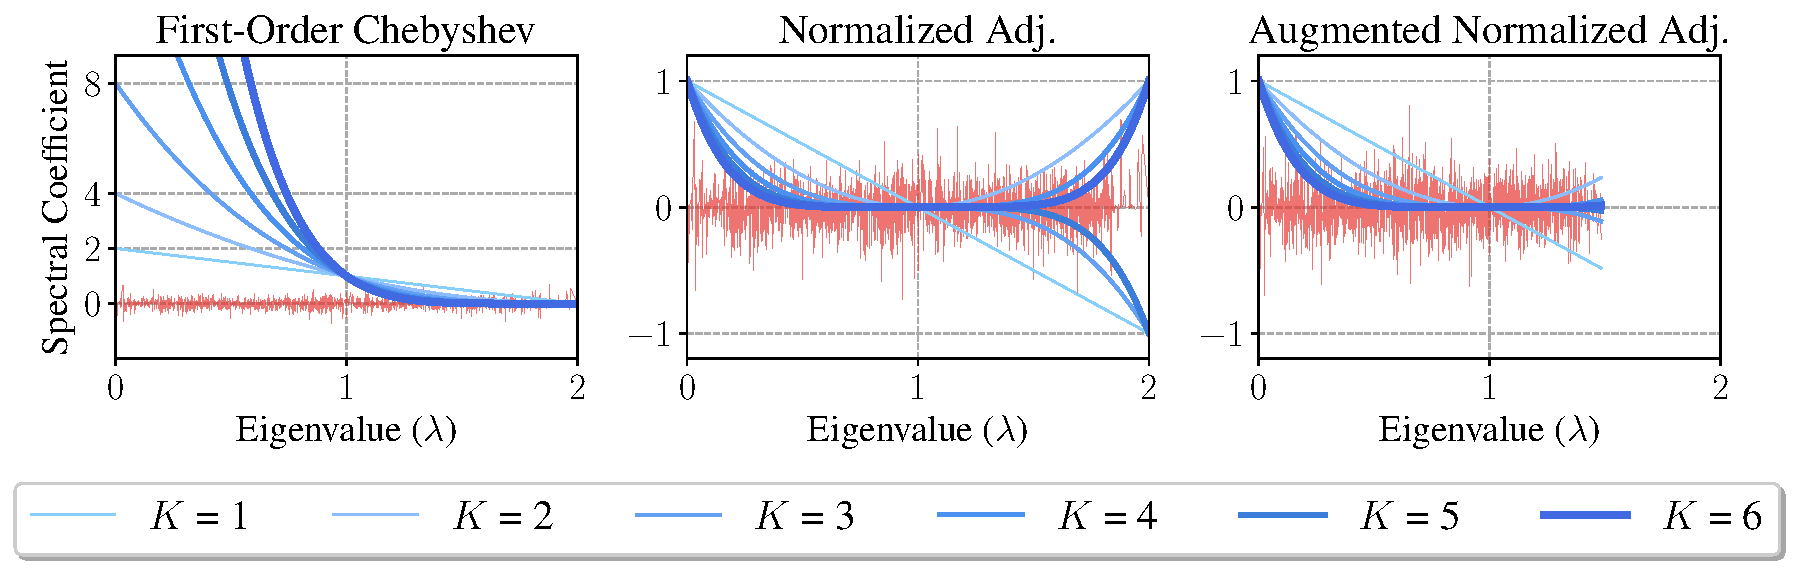
\includegraphics[width=.8\linewidth]{figures/s_filters_new2.pdf}
\caption{Feature ({\color{myred}red}) and filters ({\color{myblue}blue}) spectral coefficients for different propagation matrices on Cora dataset ($3$rd feature).}
\label{fig:s_filters}
\end{figure*}

\subsection{\method{} and Low-Pass Filtering}
The initial first-order Chebyshev filter derived in GCNs corresponds to the propagation matrix $\rmS_{\text{1-order}} = \rmI + \rmD^{-1/2} \rmA \rmD^{-1/2}$ (see \autoref{eq:first-order-cheby}). Since the normalized Laplacian is $\boldsymbol{\Delta}_{\text{sym}} = \rmI - \rmD^{-1/2} \rmA \rmD^{-1/2}$, then $\rmS_{\text{1-order}} = 2\rmI - \boldsymbol{\Delta}_{\text{sym}}$. Therefore, feature propagation with $\rmS_{\text{1-order}}^K$ implies filter coefficients $\hat{g}_i = \hat{g}(\lambda_i) = (2 - \lambda_i)^K$, where $\lambda_i$ denotes the eigenvalues of $\boldsymbol{\Delta}_{\text{sym}}$. \autoref{fig:s_filters} illustrates the filtering operation related to $\rmS_{\text{1-order}}$ for a varying number of propagation steps $K \in \{1,\dots, 6\}$. As one may observe, high powers of $\rmS_{\text{1-order}}$ lead to exploding filter coefficients and undesirably over-amplify signals at frequencies $\lambda_i < 1$.


To tackle potential numerical issues associated with the first-order Chebyshev filter, \citet{gcn} propose the \textit{renormalization trick}. Basically, it consists of replacing $\rmS_{\text{1-order}}$ by the normalized adjacency matrix after adding self-loops for all nodes. We call the resulting propagation matrix the augmented normalized adjacency matrix $\tilde{\rmS}_{\text{adj}} = \tilde{\rmD}^{-1/2}\tilde{\rmA}\tilde{\rmD}^{-1/2}$, where $\tilde{\rmA}=\rmA+\rmI$ and $\tilde{\rmD}=\rmD+\rmI$. Correspondingly, we define the augmented normalized Laplacian $\tilde{\boldsymbol{\Delta}}_{\text{sym}} = \rmI -  \tilde{\rmD}^{-1/2}\tilde{\rmA}\tilde{\rmD}^{-1/2}$. Thus, we can describe the spectral filters associated with $\tilde{\rmS}_{\text{adj}}$ as a polynomial of the eigenvalues of the underlying Laplacian, i.e.,  $\hat{g}(\tilde{\lambda}_i) = (1 - \tilde{\lambda}_i)^K$, where $\tilde{\lambda}_i$ are eigenvalues of $\tilde{\boldsymbol{\Delta}}_{\text{sym}}$.


We now analyze the spectrum of $\tilde{\boldsymbol{\Delta}}_{\text{sym}}$ and show that adding self-loops to graphs shrinks the spectrum (eigenvalues) of the corresponding normalized Laplacian.

\begin{theorem}\label{thm:Lapla_eig_shrink} Let $\rmA$ be the adjacency matrix of an undirected, weighted, simple graph $\mathcal{G}$ without isolated nodes and with corresponding degree matrix $\rmD$. Let $\tilde{\rmA} = \rmA + \gamma \rmI$, such that $\gamma > 0$, be the augmented adjacency matrix with corresponding degree matrix $\tilde{\rmD}$. Also, let $\lambda_1$ and $\lambda_n$ denote the smallest and largest eigenvalues of $\boldsymbol{\Delta}_{\text{sym}}=\rmI -  \rmD^{-1/2}\rmA\rmD^{-1/2}$; similarly, let $\tilde{\lambda}_1$ and $\tilde{\lambda}_n$ be the smallest and largest eigenvalues of $\tilde{\boldsymbol{\Delta}}_{\text{sym}}=\rmI -  \tilde{\rmD}^{-1/2}\tilde{\rmA}\tilde{\rmD}^{-1/2}$. We have that
\begin{equation}
0 = \lambda_1 = \tilde{\lambda}_1 < \tilde{\lambda}_n < \lambda_n. \label{eq:corollary_aug_laplacian}
\end{equation}
\end{theorem}
%
\autoref{thm:Lapla_eig_shrink} shows that the largest eigenvalue of the normalized graph Laplacian becomes smaller after adding self-loops $\gamma > 0$ (see supplementary materials for the proof).

\autoref{fig:s_filters} depicts the filtering operations associated with the normalized adjacency $\rmS_{\text{adj}} = \rmD^{-1/2}\rmA\rmD^{-1/2}$ and its augmented variant $\tilde{\rmS}_{\text{adj}} =  \tilde{\rmD}^{-1/2}\tilde{\rmA}\tilde{\rmD}^{-1/2}$ on the Cora dataset~\citep{sen2008collective}. Feature propagation with $\rmS_{\text{adj}}$ corresponds to filters $g(\lambda_i) = (1-\lambda_i)^K$ in the spectral range $[0, 2]$; therefore odd powers of $\rmS_{\text{adj}}$ yield negative filter coefficients at frequencies $\lambda_i > 1$. By adding self-loops ($\tilde{\rmS}_{\text{adj}}$), the largest eigenvalue shrinks from $2$ to approximately $1.5$ and then eliminates the effect of negative coefficients. Moreover, this scaled spectrum allows the filter defined by taking powers $K>1$ of $\tilde{\rmS}_{\text{adj}}$ to act as a low-pass-type filters. In supplementary material, we empirically evaluate different choices for the propagation matrix.